\def\ReportNumber{3}
\def\ReportName{Magnetoquasistatic analysis}
\documentclass[11pt,a4paper]{article}
\usepackage[T1]{fontenc}
\usepackage[utf8]{inputenc}
\usepackage{newtxtext,newtxmath,microtype}
\usepackage[margin=21mm,headheight=14pt]{geometry}
\usepackage{booktabs,tabularx,array,amsmath,graphicx,float,caption}
\usepackage{xcolor,fancyhdr,lastpage,listings}
\usepackage[hidelinks]{hyperref}
\definecolor{accent}{HTML}{254C58}
% Original question wording: NMES Assignment 2026, Sections 1--3.
% Line-wrap hyphenation is removed; mathematical notation is typeset in LaTeX.
\usepackage{tcolorbox}
\newcommand{\assignmentquestion}[1]{%
  \begin{tcolorbox}[colback=accent!4,colframe=accent!65,
    boxrule=0.4pt,leftrule=2pt,arc=0pt,boxsep=0pt,
    left=7pt,right=7pt,top=5pt,bottom=5pt,
    before skip=0pt,after skip=8pt,fontupper=\small]
  \textbf{Assignment question.} #1
  \end{tcolorbox}%
}
\newcommand{\questionfiles}[1]{%
  \par\smallskip{\footnotesize\color{accent}
  \textbf{Files / results (relative to Source-code).} #1\par}\medskip
}
\newcommand{\QuestionOneOne}{%
Describe your cable: construction, dimensions, materials, rated voltage, rated
current (ampacity) and the laying conditions for which that rating is given
(burial depth, soil thermal resistivity, ambient temperature, arrangement).
Give a table of electromagnetic and thermal properties with a source for each value.}
\newcommand{\QuestionOneTwo}{%
Choose the environment consistently with the datasheet rating conditions,
and justify its properties.}
\newcommand{\QuestionOneThree}{%
State the sheath bonding you assume: single-point bonded (no net sheath current)
or solidly bonded (circulating sheath currents allowed), and how the armour
and pipe are connected. This choice strongly affects the losses in Section 3.}
\newcommand{\QuestionOneFour}{%
State the excitation you impose: phase-to-ground voltage and phase current,
as peak phasors, with the phase sequence (see the conventions in Appendix A).}
\newcommand{\QuestionTwoOne}{%
Define your computational domain, the equations solved and the boundary
conditions. Where do you truncate the domain, and why? Discuss the role of
the grounded screens: which regions actually influence the field in the insulation?}
\newcommand{\QuestionTwoTwo}{%
Can you simplify the geometry of your cable without degrading the precision
(e.g. disregard details in the geometrical description)? Quantify the effect
of each simplification.}
\newcommand{\QuestionTwoThree}{%
How do the results vary with the mesh refinement? Plot the maximum field in
the insulation and the capacitance versus the number of degrees of freedom,
and identify where local refinement is needed.}
\newcommand{\QuestionTwoFour}{%
Define the admissible field strength at the conductor screen and at the core
screen from the datasheet (or, if absent, from a cited reference).
Is the healthy cable within these limits?}
\newcommand{\QuestionTwoFive}{%
Add a defect to the insulation of your cable. State its nature (e.g. gas void,
water tree, protrusion of the semiconducting screen), its properties, size and
position, and discuss what a defect in a 2D cross-section represents in 3D.
Compare the field with and without defect along a radial cut.
Does the cable withstand the defect?}
\newcommand{\QuestionTwoSix}{%
Compute the resistive and displacement current densities in the cable.
Is current conservation satisfied? Which current dominates in each material, and why?}
\newcommand{\QuestionTwoSeven}{%
Compute the per-unit-length capacitance (\(\mu\mathrm{F/km}\)) and compare with
the analytical value (13) and with the datasheet. State the assumptions of the
analytical formula (in particular, how the semiconducting layers are treated).
Does the capacitance vary with frequency? Why (not)?}
\newcommand{\QuestionTwoEight}{%
Propose an improvement of the cable design with respect to the electric stress,
and support it quantitatively.}
\newcommand{\QuestionThreeOne}{%
Define your computational domain, the equations solved and the boundary conditions.
Where do you truncate the domain, and why? How do you impose the currents in the phase conductors?}
\newcommand{\QuestionThreeTwo}{%
\textbf{Conductor model.} Compare the skin depth in the conductor with its radius.
Model the phase conductors (a) as stranded conductors (imposed uniform current density)
and (b) as massive conductors (imposed net current, eddy currents allowed).
Which assumption is more realistic for your cable, and how does it affect the results?}
\newcommand{\QuestionThreeThree}{%
\textbf{Bonding.} Implement the bonding assumed in Q1.3 with global quantities
(net current and voltage per unit length in the sheaths, armour and pipe).
Explain why using only \(\mathbf j=-\mathrm i\omega\sigma\mathbf a\)
in these regions does not correspond to a well-defined bonding condition.}
\newcommand{\QuestionThreeFour}{%
Can you simplify the geometry without degrading the precision?
Are the simplifications of Section 2 still valid here?}
\newcommand{\QuestionThreeFive}{%
Check the mesh quality and refine where needed (element size compared with the
skin depth in each conducting region). How do losses, resistance and inductance
vary with the mesh refinement?}
\newcommand{\QuestionThreeSix}{%
Get the magnetic flux density (or induction) in and around your cable.}
\newcommand{\QuestionThreeSeven}{%
Get the current density in the conducting parts of your cable.}
\newcommand{\QuestionThreeEight}{%
Get the time-averaged Joule losses (kW/km) in each conducting part
(conductors, sheaths, armour, pipe, environment).}
\newcommand{\QuestionThreeNine}{%
Get the per-unit-length AC resistance (\(\Omega/\mathrm{km}\)), defined from
the total losses. Compare it with the DC resistance and with the datasheet.
Separate the contributions of skin/proximity effect and of sheath/armour losses.}
\newcommand{\QuestionThreeTen}{%
Get the per-unit-length inductance (mH/km). How do you define it for a
three-phase system? Does it vary with frequency? Compare with the datasheet.}
\newcommand{\QuestionThreeEleven}{%
Propose a design change that reduces the losses, and support it quantitatively.}

\pagestyle{fancy}\fancyhf{}
\fancyhead[L]{\small FE for Electromagnetic Fields -- Kutikuppala, Lefebure, Miseur}
\fancyhead[R]{\small NKT 33 kV, 185 + 50 mm\textsuperscript{2}}
\fancyfoot[L]{\small Section \ReportNumber\ -- \ReportName}
\fancyfoot[R]{\small\thepage\,/\,\pageref{LastPage}}
\renewcommand{\headrulewidth}{0.3pt}
\setlength{\parindent}{0pt}\setlength{\parskip}{5pt}
\setlength{\emergencystretch}{2em}
\setlength{\tabcolsep}{5pt}\renewcommand{\arraystretch}{1.13}
\captionsetup{font=small,labelfont=bf,skip=5pt}
\newcolumntype{Y}{>{\raggedright\arraybackslash}X}
\newcommand{\file}[1]{\href{../Source-code/#1}{\nolinkurl{#1}}}
\newcommand{\setupfile}[1]{\file{Cable-selection-and-model-setup/#1}}
\newcommand{\efile}{\file{Electrodynamic-analysis/cable.pro}}
\newcommand{\mfile}{\file{Magnetothermal-analysis/cable.pro}}
\newcommand{\runall}{\href{../run_all.sh}{\nolinkurl{run_all.sh}}}
\newcommand{\runE}{\texttt{getdp cable.pro -msh}\ \path{../Cable-selection-and-model-setup/cable.msh}\ \texttt{-solve Electrodynamics}}
\newcommand{\codeguide}[3]{\par\smallskip
 {\small\bfseries\color{accent}Code guide}\par\nobreak
 \begingroup\small\setlength{\tabcolsep}{0pt}
 \begin{tabularx}{\linewidth}{@{}p{14mm}Y@{}}
 \textbf{Files} & #1\\[2pt]
 \textbf{Run} & #2\\[2pt]
 \textbf{Check} & #3
 \end{tabularx}\par\endgroup\medskip}
\newcommand{\pending}{\textbf{Status: implementation still required.} }
\newcommand{\refurl}[2]{\href{#1}{#2}}
\lstset{basicstyle=\small\ttfamily,columns=fullflexible,keepspaces=true,
 showstringspaces=false,breaklines=true,upquote=true,
 backgroundcolor=\color{accent!4},frame=none,
 xleftmargin=5pt,xrightmargin=5pt,aboveskip=5pt,belowskip=5pt}
\hypersetup{pdftitle={Section \ReportNumber: \ReportName},
  pdfauthor={Kutikuppala Jaswanth, Lefebure Tiebert, Miseur Torre}}

\usepackage{pgfplots}\pgfplotsset{compat=1.18}
\graphicspath{{../../Slides/figures/}}
% Generated by Reports/collect_values.py. Do not edit.
\newcommand{\AmpLin}{386}
\newcommand{\Ampflat}{343}
\newcommand{\Ampflatsev}{352}
\newcommand{\Ampflatsevsp}{374}
\newcommand{\Ampflatsp}{351}
\newcommand{\Amptrefoil}{345}
\newcommand{\Amptrefoilsp}{350}
\newcommand{\AnaC}{0.197031}
\newcommand{\AnaCbare}{0.1834}
\newcommand{\AnaCthick}{0.181271}
\newcommand{\AnaDeltaAl}{11.96}
\newcommand{\AnaDeltaCu}{9.35}
\newcommand{\AnaDrop}{7}
\newcommand{\AnaEb}{5.14}
\newcommand{\AnaEi}{4.894}
\newcommand{\AnaEirms}{3.46}
\newcommand{\AnaEithick}{4.502}
\newcommand{\AnaEorms}{1.71}
\newcommand{\AnaEvoid}{6.20}
\newcommand{\AnaEzero}{4.34}
\newcommand{\AnaIch}{1.179}
\newcommand{\AnaJc}{\ensuremath{4.89\cdot10^{-12}}}
\newcommand{\AnaJd}{0.0340}
\newcommand{\AnaLgap}{0.4043}
\newcommand{\AnaLtouch}{0.4019}
\newcommand{\AnaRatio}{\ensuremath{1.44\cdot10^{-10}}}
\newcommand{\AnaWd}{0.022}
\newcommand{\AnaWdShare}{0.09}
\newcommand{\Bmax}{15.6}
\newcommand{\Bsingle}{13.4}
\newcommand{\Cdefect}{0.197000}
\newcommand{\Cdefectfine}{0.196999}
\newcommand{\Cffive}{0.197032}
\newcommand{\Cfhund}{0.197032}
\newcommand{\Cfthou}{0.197032}
\newcommand{\Cgap}{0.197032}
\newcommand{\Cgapcoarse}{0.197044}
\newcommand{\Cgapfine}{0.197031}
\newcommand{\CondShare}{94}
\newcommand{\ConvRate}{0.22}
\newcommand{\Cqdefect}{0.196937}
\newcommand{\Cqdefectfine}{0.196935}
\newcommand{\Cqffive}{0.197032}
\newcommand{\Cqfhund}{0.197032}
\newcommand{\Cqfthou}{0.197032}
\newcommand{\Cqgap}{0.197032}
\newcommand{\Cqgapcoarse}{0.197044}
\newcommand{\Cqgapfine}{0.197031}
\newcommand{\Cqthick}{0.181272}
\newcommand{\Cqtouching}{0.197032}
\newcommand{\Cthick}{0.181272}
\newcommand{\Ctouching}{0.197032}
\newcommand{\Dofsdefect}{65\,900}
\newcommand{\Dofsdefectfine}{265\,156}
\newcommand{\Dofsffive}{64\,884}
\newcommand{\Dofsfhund}{64\,884}
\newcommand{\Dofsfthou}{64\,884}
\newcommand{\Dofsgap}{64\,884}
\newcommand{\Dofsgapcoarse}{16\,100}
\newcommand{\Dofsgapfine}{261\,058}
\newcommand{\Dofsthick}{76\,210}
\newcommand{\Dofstouching}{64\,880}
\newcommand{\EddyFE}{0.9}
\newcommand{\Edefect}{6.29}
\newcommand{\Edefectfine}{6.30}
\newcommand{\Effive}{4.873}
\newcommand{\Efhund}{4.873}
\newcommand{\Efthou}{4.873}
\newcommand{\Egap}{4.873}
\newcommand{\Egapcoarse}{4.846}
\newcommand{\Egapfine}{4.885}
\newcommand{\Ethick}{4.474}
\newcommand{\Etouching}{4.872}
\newcommand{\Hrad}{5.2}
\newcommand{\Ibalance}{\ensuremath{4\cdot10^{-14}}}
\newcommand{\IchFE}{1.179}
\newcommand{\IecAmp}{351}
\newcommand{\IecIs}{56.8}
\newcommand{\IecLam}{5.52}
\newcommand{\IecLamHot}{3.6}
\newcommand{\IecPc}{60.55}
\newcommand{\IecPcHot}{76.8}
\newcommand{\IecPs}{3.34}
\newcommand{\IecPsHot}{2.76}
\newcommand{\IecPt}{63.89}
\newcommand{\IecRac}{0.1739}
\newcommand{\IecRacHot}{0.2164}
\newcommand{\IecRcond}{0.16475}
\newcommand{\IecRcondHot}{0.2089}
\newcommand{\IecRs}{0.3448}
\newcommand{\IecTfour}{2.236}
\newcommand{\IecTheta}{89.2}
\newcommand{\IecThetaS}{77}
\newcommand{\IecTone}{0.476}
\newcommand{\IecTthree}{0.104}
\newcommand{\IecU}{46.5}
\newcommand{\IecUs}{19.9}
\newcommand{\IecX}{0.0568}
\newcommand{\IecYp}{0.15}
\newcommand{\IecYs}{0.31}
\newcommand{\IecYsp}{0.46}
\newcommand{\Ioneflat}{341}
\newcommand{\Ioneflatsev}{353}
\newcommand{\Ioneflatsevsp}{381}
\newcommand{\Ioneflatsp}{351}
\newcommand{\Ionetrefoil}{344}
\newcommand{\Ionetrefoilsp}{350}
\newcommand{\IratioFE}{\ensuremath{1.44\cdot10^{-10}}}
\newcommand{\IsPeak}{79}
\newcommand{\IsSum}{0.15}
\newcommand{\Isbase}{55.5}
\newcommand{\Isbox}{55.9}
\newcommand{\Iscoarse}{54.9}
\newcommand{\Isfdc}{0.0}
\newcommand{\Isffive}{5.7}
\newcommand{\Isfhund}{267.6}
\newcommand{\Isfine}{55.8}
\newcommand{\Isflat}{60.9}
\newcommand{\IsflatIone}{60.0}
\newcommand{\Isflatsev}{95.4}
\newcommand{\IsflatsevIone}{95.9}
\newcommand{\Isflatsevsp}{0.0}
\newcommand{\IsflatsevspIone}{0.0}
\newcommand{\Isflatsp}{0.0}
\newcommand{\IsflatspIone}{0.0}
\newcommand{\Islin}{55.5}
\newcommand{\Isliniso}{55.5}
\newcommand{\Isnl}{45.4}
\newcommand{\Isnlcoarse}{45.0}
\newcommand{\Isnldomforty}{45.4}
\newcommand{\Isnldomten}{45.4}
\newcommand{\Isnlfine}{45.5}
\newcommand{\Isnlhfive}{45.2}
\newcommand{\Isnlhtwenty}{45.5}
\newcommand{\Isnliso}{45.6}
\newcommand{\Issingle}{0.0}
\newcommand{\Isstranded}{55.6}
\newcommand{\Isstrandedfhund}{268.1}
\newcommand{\Istouching}{54.9}
\newcommand{\Istrefoil}{45.4}
\newcommand{\IstrefoilIone}{45.0}
\newcommand{\Istrefoilsp}{0.0}
\newcommand{\IstrefoilspIone}{0.0}
\newcommand{\Javg}{2.88}
\newcommand{\JcFE}{\ensuremath{4.87\cdot10^{-12}}}
\newcommand{\JdFE}{0.0339}
\newcommand{\Jmax}{3.07}
\newcommand{\Jscreen}{1.6}
\newcommand{\LamFE}{6.1}
\newcommand{\Lbase}{0.3943}
\newcommand{\Lbox}{0.3955}
\newcommand{\Lcoarse}{0.3922}
\newcommand{\Lfdc}{0.4010}
\newcommand{\Lffive}{0.4010}
\newcommand{\Lfhund}{0.2616}
\newcommand{\Lfine}{0.3952}
\newcommand{\Lflat}{0.4331}
\newcommand{\LflatIone}{0.4328}
\newcommand{\Lflatsev}{0.5722}
\newcommand{\LflatsevIone}{0.5724}
\newcommand{\Lflatsevsp}{0.6061}
\newcommand{\LflatsevspIone}{0.6061}
\newcommand{\Lflatsp}{0.4437}
\newcommand{\LflatspIone}{0.4437}
\newcommand{\Llin}{0.3943}
\newcommand{\Lliniso}{0.3943}
\newcommand{\Lnl}{0.3965}
\newcommand{\Lnlcoarse}{0.3944}
\newcommand{\Lnldomforty}{0.3965}
\newcommand{\Lnldomten}{0.3965}
\newcommand{\Lnlfine}{0.3975}
\newcommand{\Lnlhfive}{0.3966}
\newcommand{\Lnlhtwenty}{0.3965}
\newcommand{\Lnliso}{0.3965}
\newcommand{\Lsingle}{0.4003}
\newcommand{\Lstranded}{0.3947}
\newcommand{\Lstrandedfhund}{0.2670}
\newcommand{\Lterm}{0.3945}
\newcommand{\Ltouching}{0.3923}
\newcommand{\Ltrefoil}{0.3965}
\newcommand{\LtrefoilIone}{0.3965}
\newcommand{\Ltrefoilsp}{0.4006}
\newcommand{\LtrefoilspIone}{0.4006}
\newcommand{\MDofsbase}{295\,294}
\newcommand{\MDofsbox}{297\,138}
\newcommand{\MDofscoarse}{75\,856}
\newcommand{\MDofsfdc}{295\,294}
\newcommand{\MDofsffive}{295\,294}
\newcommand{\MDofsfhund}{295\,294}
\newcommand{\MDofsfine}{1\,169\,120}
\newcommand{\MDofsflat}{243\,780}
\newcommand{\MDofsflatIone}{243\,780}
\newcommand{\MDofsflatsev}{253\,538}
\newcommand{\MDofsflatsevIone}{253\,538}
\newcommand{\MDofsflatsevsp}{253\,538}
\newcommand{\MDofsflatsevspIone}{253\,538}
\newcommand{\MDofsflatsp}{243\,780}
\newcommand{\MDofsflatspIone}{243\,780}
\newcommand{\MDofslin}{295\,294}
\newcommand{\MDofsliniso}{295\,294}
\newcommand{\MDofsnl}{295\,294}
\newcommand{\MDofsnlcoarse}{75\,856}
\newcommand{\MDofsnldomforty}{295\,294}
\newcommand{\MDofsnldomten}{295\,294}
\newcommand{\MDofsnlfine}{1\,169\,120}
\newcommand{\MDofsnlhfive}{295\,294}
\newcommand{\MDofsnlhtwenty}{295\,294}
\newcommand{\MDofsnliso}{295\,294}
\newcommand{\MDofssingle}{295\,294}
\newcommand{\MDofsstranded}{295\,288}
\newcommand{\MDofsstrandedfhund}{295\,288}
\newcommand{\MDofstouching}{292\,266}
\newcommand{\MDofstrefoil}{295\,294}
\newcommand{\MDofstrefoilIone}{295\,294}
\newcommand{\MDofstrefoilsp}{295\,294}
\newcommand{\MDofstrefoilspIone}{295\,294}
\newcommand{\MeshBadGap}{0}
\newcommand{\MeshBadTouch}{24}
\newcommand{\MeshQminGap}{0.575}
\newcommand{\MeshQminTouch}{0.020}
\newcommand{\MeshTriGap}{297\,943}
\newcommand{\MeshTriTouch}{294\,915}
\newcommand{\MeshXlpeGap}{22\,228}
\newcommand{\MeshXlpeTouch}{22\,222}
\newcommand{\Nitflat}{10}
\newcommand{\NitflatIone}{10}
\newcommand{\Nitflatsev}{9}
\newcommand{\NitflatsevIone}{9}
\newcommand{\Nitflatsevsp}{10}
\newcommand{\NitflatsevspIone}{11}
\newcommand{\Nitflatsp}{10}
\newcommand{\NitflatspIone}{10}
\newcommand{\Nitlin}{1}
\newcommand{\Nitliniso}{1}
\newcommand{\Nitnl}{10}
\newcommand{\Nitnlcoarse}{10}
\newcommand{\Nitnldomforty}{10}
\newcommand{\Nitnldomten}{10}
\newcommand{\Nitnlfine}{10}
\newcommand{\Nitnlhfive}{10}
\newcommand{\Nitnlhtwenty}{10}
\newcommand{\Nitnliso}{10}
\newcommand{\Nittrefoil}{10}
\newcommand{\NittrefoilIone}{10}
\newcommand{\Nittrefoilsp}{10}
\newcommand{\NittrefoilspIone}{10}
\newcommand{\NktL}{0.382}
\newcommand{\PcPhase}{20.18}
\newcommand{\Pcbase}{60.55}
\newcommand{\Pcbox}{60.55}
\newcommand{\Pccoarse}{60.58}
\newcommand{\Pcfdc}{60.28}
\newcommand{\Pcffive}{60.28}
\newcommand{\Pcfhund}{75.76}
\newcommand{\Pcfine}{60.54}
\newcommand{\Pcflat}{77.44}
\newcommand{\PcflatIone}{72.36}
\newcommand{\Pcflatsev}{76.02}
\newcommand{\PcflatsevIone}{77.69}
\newcommand{\Pcflatsevsp}{73.63}
\newcommand{\PcflatsevspIone}{91.14}
\newcommand{\Pcflatsp}{76.37}
\newcommand{\PcflatspIone}{77.04}
\newcommand{\PcircFE}{3.16}
\newcommand{\Pclin}{60.55}
\newcommand{\Pcliniso}{60.55}
\newcommand{\Pcnl}{77.58}
\newcommand{\Pcnlcoarse}{77.38}
\newcommand{\Pcnldomforty}{77.59}
\newcommand{\Pcnldomten}{77.51}
\newcommand{\Pcnlfine}{77.65}
\newcommand{\Pcnlhfive}{77.92}
\newcommand{\Pcnlhtwenty}{77.40}
\newcommand{\Pcnliso}{77.21}
\newcommand{\Pcsingle}{60.55}
\newcommand{\Pcstranded}{60.26}
\newcommand{\Pcstrandedfhund}{60.26}
\newcommand{\Pctouching}{60.55}
\newcommand{\Pctrefoil}{77.58}
\newcommand{\PctrefoilIone}{74.07}
\newcommand{\Pctrefoilsp}{76.94}
\newcommand{\PctrefoilspIone}{76.94}
\newcommand{\PdInception}{16}
\newcommand{\PhaseSym}{0.0004}
\newcommand{\Psbase}{3.68}
\newcommand{\Psbox}{3.74}
\newcommand{\Pscoarse}{3.59}
\newcommand{\Psfdc}{0.00}
\newcommand{\Psffive}{0.04}
\newcommand{\Psfhund}{81.84}
\newcommand{\Psfine}{3.72}
\newcommand{\Psflat}{5.01}
\newcommand{\PsflatIone}{4.81}
\newcommand{\Psflatsev}{12.34}
\newcommand{\PsflatsevIone}{12.51}
\newcommand{\Psflatsevsp}{0.05}
\newcommand{\PsflatsevspIone}{0.05}
\newcommand{\Psflatsp}{0.41}
\newcommand{\PsflatspIone}{0.41}
\newcommand{\Pslin}{3.68}
\newcommand{\Psliniso}{3.68}
\newcommand{\Psnl}{3.03}
\newcommand{\Psnlcoarse}{2.96}
\newcommand{\Psnldomforty}{3.03}
\newcommand{\Psnldomten}{3.03}
\newcommand{\Psnlfine}{3.06}
\newcommand{\Psnlhfive}{3.02}
\newcommand{\Psnlhtwenty}{3.04}
\newcommand{\Psnliso}{3.04}
\newcommand{\Pssingle}{0.52}
\newcommand{\Psstranded}{3.70}
\newcommand{\Psstrandedfhund}{83.03}
\newcommand{\Pstouching}{3.62}
\newcommand{\Pstrefoil}{3.03}
\newcommand{\PstrefoilIone}{2.95}
\newcommand{\Pstrefoilsp}{0.43}
\newcommand{\PstrefoilspIone}{0.43}
\newcommand{\Ptbase}{64.23}
\newcommand{\Ptbox}{64.30}
\newcommand{\Ptcoarse}{64.17}
\newcommand{\Ptfdc}{60.28}
\newcommand{\Ptffive}{60.32}
\newcommand{\Ptfhund}{157.60}
\newcommand{\Ptfine}{64.27}
\newcommand{\Ptflat}{82.45}
\newcommand{\PtflatIone}{77.17}
\newcommand{\Ptflatsev}{88.36}
\newcommand{\PtflatsevIone}{90.20}
\newcommand{\Ptflatsevsp}{73.68}
\newcommand{\PtflatsevspIone}{91.20}
\newcommand{\Ptflatsp}{76.77}
\newcommand{\PtflatspIone}{77.45}
\newcommand{\Ptlin}{64.23}
\newcommand{\Ptliniso}{64.23}
\newcommand{\Ptnl}{80.61}
\newcommand{\Ptnlcoarse}{80.33}
\newcommand{\Ptnldomforty}{80.62}
\newcommand{\Ptnldomten}{80.55}
\newcommand{\Ptnlfine}{80.71}
\newcommand{\Ptnlhfive}{80.94}
\newcommand{\Ptnlhtwenty}{80.43}
\newcommand{\Ptnliso}{80.25}
\newcommand{\Ptsingle}{61.07}
\newcommand{\Ptstranded}{63.96}
\newcommand{\Ptstrandedfhund}{143.29}
\newcommand{\Pttouching}{64.17}
\newcommand{\Pttrefoil}{80.61}
\newcommand{\PttrefoilIone}{77.02}
\newcommand{\Pttrefoilsp}{77.36}
\newcommand{\PttrefoilspIone}{77.36}
\newcommand{\QsFrac}{94.6}
\newcommand{\Racbase}{0.1748}
\newcommand{\Racbox}{0.1750}
\newcommand{\Raccoarse}{0.1746}
\newcommand{\Racfdc}{0.1640}
\newcommand{\Racffive}{0.1641}
\newcommand{\Racfhund}{0.4288}
\newcommand{\Racfine}{0.1749}
\newcommand{\Racflat}{0.2244}
\newcommand{\RacflatIone}{0.2214}
\newcommand{\Racflatsev}{0.2404}
\newcommand{\RacflatsevIone}{0.2413}
\newcommand{\Racflatsevsp}{0.2005}
\newcommand{\RacflatsevspIone}{0.2097}
\newcommand{\Racflatsp}{0.2089}
\newcommand{\RacflatspIone}{0.2093}
\newcommand{\Raclin}{0.1748}
\newcommand{\Racliniso}{0.1748}
\newcommand{\Racnl}{0.2193}
\newcommand{\Racnlcoarse}{0.2186}
\newcommand{\Racnldomforty}{0.2194}
\newcommand{\Racnldomten}{0.2192}
\newcommand{\Racnlfine}{0.2196}
\newcommand{\Racnlhfive}{0.2202}
\newcommand{\Racnlhtwenty}{0.2189}
\newcommand{\Racnliso}{0.2184}
\newcommand{\Racsingle}{0.1662}
\newcommand{\Racstranded}{0.1740}
\newcommand{\Racstrandedfhund}{0.3899}
\newcommand{\Ractouching}{0.1746}
\newcommand{\Ractrefoil}{0.2193}
\newcommand{\RactrefoilIone}{0.2172}
\newcommand{\Ractrefoilsp}{0.2105}
\newcommand{\RactrefoilspIone}{0.2105}
\newcommand{\Rcbase}{0.1648}
\newcommand{\Rcbox}{0.1648}
\newcommand{\Rccoarse}{0.1648}
\newcommand{\Rcfdc}{0.1640}
\newcommand{\Rcffive}{0.1640}
\newcommand{\Rcfhund}{0.2061}
\newcommand{\Rcfine}{0.1647}
\newcommand{\Rcflat}{0.2107}
\newcommand{\RcflatIone}{0.2076}
\newcommand{\Rcflatsev}{0.2069}
\newcommand{\RcflatsevIone}{0.2078}
\newcommand{\Rcflatsevsp}{0.2004}
\newcommand{\RcflatsevspIone}{0.2096}
\newcommand{\Rcflatsp}{0.2078}
\newcommand{\RcflatspIone}{0.2082}
\newcommand{\Rclin}{0.1648}
\newcommand{\Rcliniso}{0.1648}
\newcommand{\Rcnl}{0.2111}
\newcommand{\Rcnlcoarse}{0.2105}
\newcommand{\Rcnldomforty}{0.2111}
\newcommand{\Rcnldomten}{0.2109}
\newcommand{\Rcnlfine}{0.2113}
\newcommand{\Rcnlhfive}{0.2120}
\newcommand{\Rcnlhtwenty}{0.2106}
\newcommand{\Rcnliso}{0.2101}
\newcommand{\Rcsingle}{0.1648}
\newcommand{\Rcstranded}{0.1640}
\newcommand{\Rcstrandedfhund}{0.1640}
\newcommand{\Rctouching}{0.1648}
\newcommand{\Rctrefoil}{0.2111}
\newcommand{\RctrefoilIone}{0.2089}
\newcommand{\Rctrefoilsp}{0.2094}
\newcommand{\RctrefoilspIone}{0.2094}
\newcommand{\RhoHot}{28}
\newcommand{\ScreenFE}{6.1}
\newcommand{\SkinFE}{0.45}
\newcommand{\TDofsnl}{149\,003}
\newcommand{\TcA}{92.52}
\newcommand{\TcB}{92.74}
\newcommand{\TcC}{92.74}
\newcommand{\Tcflat}{94.1}
\newcommand{\TcflatIone}{89.0}
\newcommand{\Tcflatsev}{88.7}
\newcommand{\TcflatsevIone}{90.3}
\newcommand{\Tcflatsevsp}{78.4}
\newcommand{\TcflatsevspIone}{93.5}
\newcommand{\Tcflatsp}{89.5}
\newcommand{\TcflatspIone}{90.1}
\newcommand{\Tclin}{76.7}
\newcommand{\Tcliniso}{75.8}
\newcommand{\Tcnl}{92.7}
\newcommand{\Tcnlcoarse}{91.7}
\newcommand{\Tcnldomforty}{92.8}
\newcommand{\Tcnldomten}{92.5}
\newcommand{\Tcnlfine}{93.1}
\newcommand{\Tcnlhfive}{94.2}
\newcommand{\Tcnlhtwenty}{92.0}
\newcommand{\Tcnliso}{91.2}
\newcommand{\Tctrefoil}{92.7}
\newcommand{\TctrefoilIone}{89.3}
\newcommand{\Tctrefoilsp}{90.0}
\newcommand{\TctrefoilspIone}{90.0}
\newcommand{\Tsflat}{17.42}
\newcommand{\TsflatIone}{17.27}
\newcommand{\Tsflatsev}{17.58}
\newcommand{\TsflatsevIone}{17.63}
\newcommand{\Tsflatsevsp}{17.15}
\newcommand{\TsflatsevspIone}{17.66}
\newcommand{\Tsflatsp}{17.25}
\newcommand{\TsflatspIone}{17.27}
\newcommand{\Tslin}{16.89}
\newcommand{\Tsliniso}{15.00}
\newcommand{\Tsnl}{17.37}
\newcommand{\Tsnlcoarse}{17.36}
\newcommand{\Tsnldomforty}{17.37}
\newcommand{\Tsnldomten}{17.35}
\newcommand{\Tsnlfine}{17.38}
\newcommand{\Tsnlhfive}{19.47}
\newcommand{\Tsnlhtwenty}{16.23}
\newcommand{\Tsnliso}{15.00}
\newcommand{\Tstrefoil}{17.37}
\newcommand{\TstrefoilIone}{17.26}
\newcommand{\Tstrefoilsp}{17.28}
\newcommand{\TstrefoilspIone}{17.28}
\newcommand{\Usingle}{19.5}
\newcommand{\Vmeandefect}{6.11}
\newcommand{\Vmeandefectfine}{6.14}
\newcommand{\VoidRatio}{1.42}
\newcommand{\Zrbase}{0.1748}
\newcommand{\dAmpSingle}{+5}
\newcommand{\dCana}{0.0007}
\newcommand{\dCbare}{\ensuremath{-6.9}}
\newcommand{\dCnkt}{\ensuremath{-10.4}}
\newcommand{\dCthick}{\ensuremath{-8.0}}
\newcommand{\dCtouch}{\ensuremath{9\cdot10^{-6}}}
\newcommand{\dEfine}{\ensuremath{-0.17}}
\newcommand{\dEgap}{\ensuremath{-0.43}}
\newcommand{\dEthick}{\ensuremath{-8.2}}
\newcommand{\dEtouch}{+0.014}
\newcommand{\dIs}{\ensuremath{-2.3}}
\newcommand{\dLNL}{+0.57}
\newcommand{\dLana}{\ensuremath{-1.0}}
\newcommand{\dLbox}{+0.31}
\newcommand{\dLfine}{+0.23}
\newcommand{\dLflat}{+53}
\newcommand{\dLfreq}{\ensuremath{-1.7}}
\newcommand{\dLfreqhund}{\ensuremath{-35}}
\newcommand{\dLnkt}{+2.7}
\newcommand{\dLstr}{+0.09}
\newcommand{\dLterm}{0.06}
\newcommand{\dLtouch}{+0.52}
\newcommand{\dNktMax}{+0.3}
\newcommand{\dNktMin}{\ensuremath{-3.4}}
\newcommand{\dNktflat}{\ensuremath{-2.1}}
\newcommand{\dNktflatsev}{\ensuremath{-3.4}}
\newcommand{\dNktflatsevsp}{\ensuremath{-1.6}}
\newcommand{\dNktflatsp}{+0.3}
\newcommand{\dNkttrefoil}{\ensuremath{-1.4}}
\newcommand{\dNkttrefoilsp}{\ensuremath{-0.0}}
\newcommand{\dPcNL}{+28.1}
\newcommand{\dPcirc}{\ensuremath{-5}}
\newcommand{\dPsNL}{\ensuremath{-17.7}}
\newcommand{\dPsfine}{+1.2}
\newcommand{\dPstouch}{+1.7}
\newcommand{\dPtNL}{+25.5}
\newcommand{\dPtSingle}{\ensuremath{-4.9}}
\newcommand{\dRacNL}{+25.5}
\newcommand{\dRacSingle}{\ensuremath{-4.9}}
\newcommand{\dRacbox}{+0.10}
\newcommand{\dRacfine}{+0.06}
\newcommand{\dRactouch}{+0.09}
\newcommand{\dRcstr}{\ensuremath{-0.48}}
\newcommand{\dRcstrhund}{\ensuremath{-20}}
\newcommand{\dTIone}{3.5}
\newcommand{\dTcAlow}{0.2}
\newcommand{\dTcBC}{0.00}
\newcommand{\dTcCoarse}{\ensuremath{-1.0}}
\newcommand{\dTcDom}{+0.07}
\newcommand{\dTcDomten}{\ensuremath{-0.27}}
\newcommand{\dTcFine}{+0.3}
\newcommand{\dTcIso}{1.6}
\newcommand{\dTcNL}{+16.0}
\newcommand{\dTcNkt}{+2.7}
\newcommand{\dTfiller}{2.1}
\newcommand{\dToneThick}{6.5}
\newcommand{\dTsemi}{0.8}
\newcommand{\dTsurf}{2.4}
\newcommand{\dTthick}{0.8}

\begin{document}
All results: three phases at 350 A RMS, 50 Hz, 20\(^\circ\)C conductivities,
0.5 mm gap, default mesh (\texttt{MeshFactor} 1), massive aluminium and both-end
bonded screens unless stated otherwise. Peak phasors are used inside GetDP;
losses are time averages and currents are reported RMS. Every Section 3 result uses the
resolution \texttt{Magnetodynamics} of \mfile\ (select it in the GetDP panel; the default
\texttt{MagnetoThermal} is Section 4). The exact command of each case is in \runall.

\section*{Q3.1 Domain, equations, boundary conditions and sources}
\assignmentquestion{\QuestionThreeOne}
\textbf{Domain.} The whole shared mesh: three cables with all eight layers and
the \(0.6\times0.6~\mathrm m\) soil box. Unlike Section 2, the copper screens do
not shield the magnetic field, so all cables, the space between them and the
surrounding soil must be in the domain.
Conducting (massive) regions \(\Omega_c\): aluminium 21--23 and copper 71--73.
Semiconductors (\(\sigma=2\,10^{-3}\) S/m), XLPE, PE, fillers and soil
(\(\sigma=10^{-2}\) S/m, \(\delta\approx712\) m at 50 Hz) carry negligible eddy
current and are modelled with \(\sigma=0\). All materials have \(\mu_r=1\).

\textbf{Equations.} With \(\mathbf a=a_z(x,y)\mathbf e_z\), \(\mathbf b=\nabla\times\mathbf a\):
\[
 \nabla\times(\nu\nabla\times\mathbf a)=\mathbf j,\qquad
 \mathbf j=-\sigma\,(j\omega\mathbf a+\mathbf u_r)\ \text{in }\Omega_c,\qquad
 \mathbf j=\mathbf j_s=\frac{\hat I_k}{A_k}\mathbf e_z\ \text{(stranded option)}.
\]
\(\mathbf u_r=\nabla v\) is constant along \(z\) in each massive region (one unknown
per region, \texttt{BF\_RegionZ}). Testing with that basis function gives the
circuit relation \(\int_{\Omega_m}j_z\,dA=I_m\): every massive region needs either
its net current \(I_m\) or its voltage per unit length \(U_m\) imposed.
The displacement current is neglected (\(\omega\varepsilon\ll\sigma\) in metals; the
radial charging current of Section 2 is 1.2 A/km versus 350 A axial).

\textbf{Boundary condition and truncation.} \(a_z=0\) on the box edge (group 120).
The phase currents are balanced (\(\sum\hat I_k=0\)) and the screen currents
nearly so (\(|\sum \hat I_{s}|=0.14~\mathrm A\) peak), so the far field decays like a
multipole, \(\propto1/r^2\). The edge is at 0.3 m, about 7 cable spacings.
Doubling the half-box to 0.6 m changes \(L\) by
+0.30\% and \(R_{AC}\) by +0.10\% (Q3.5): the truncation is adequate.

\textbf{Currents.} Massive model: the net current of each aluminium region is imposed
as a global constraint, \(\hat I_k=\sqrt2\,350\,e^{-j2\pi k/3}\) A; the current
distribution inside (skin/proximity) is free. Stranded option: a uniform
\(\hat{\mathbf j}_s=\hat I_k/A_k\) is imposed and the conductors leave \(\Omega_c\).

\codeguide{\mfile: \texttt{Group}, \texttt{Constraint}, \texttt{FunctionSpace},
\texttt{Formulation}. \setupfile{cable.geo}: physical groups (README table).}
{In Gmsh open \mfile\ and press \textbf{Run} (resolution \texttt{Magnetodynamics}).}
{Output panel: losses, \(R\), \(L\). \texttt{res/currents\_A.dat}: imposed phase currents,
then the three induced screen currents.}

\newpage
\section*{Q3.2 Conductor model: massive versus stranded}
\assignmentquestion{\QuestionThreeTwo}
At 50 Hz, \(\delta=\sqrt{2/(\omega\mu_0\sigma)}\):
\(\delta_{\rm Al}=11.96~\mathrm{mm}\) for \(r_c=7.4~\mathrm{mm}\) (\(r_c/\delta=0.62\)),
\(\delta_{\rm Cu}=9.23~\mathrm{mm}\) for a 0.45 mm screen. Skin effect is weak.
\begin{center}\small
\begin{tabular}{@{}lrrrr@{}}\toprule
50 Hz & \(P_{\rm cond}\) [kW/km] & \(P_{\rm screen}\) [kW/km] & \(R_{\rm cond}\) [\(\Omega\)/km] & \(L\) [mH/km]\\\midrule
(a) Stranded, uniform \(J\) & \Pcstranded & \Psstranded & \Rcstranded & \Lstranded\\
(b) Massive, eddy currents & \Pcbase & \Psbase & \Rcbase & \Lbase\\\midrule
500 Hz, stranded & \Pcstrandedfhund & \Psstrandedfhund & \Rcstrandedfhund & \Lstrandedfhund\\
500 Hz, massive & \Pcfhund & \Psfhund & \Rcfhund & \Lfhund\\\bottomrule
\end{tabular}
\end{center}
\textbf{More realistic: massive.} NKT specifies a \emph{solid} circular aluminium
conductor, so eddy currents can flow inside it. The stranded model reproduces
exactly \(R_{DC}\) (its value is 0.02\% below 0.164 only because the 12-arc
polygon has 0.02\% less area than the circle). At 50 Hz the massive model gives
\(R_{\rm cond}/R_{DC,\rm FE}-1=0.45\%\) (skin + proximity, with \(R_{DC,\rm FE}=\)\,\Racfdc\ from
the 0.01 Hz run); the IEC 60287 factors give \(y_s+y_p=0.0031+0.0015=0.46\%\) [IEC].
\(L\) changes by only 0.1\% (the stranded model has slightly more internal inductance).
At 500 Hz (\(r_c/\delta=1.97\)) the difference becomes large (\(+26\%\) in
\(R_{\rm cond}\)): the stranded model is then not acceptable for a solid conductor.

\codeguide{\mfile: \texttt{Flag\_Conductor}, \texttt{DomainS0\_Mag}, \texttt{js0[]}.}
{Gmsh: \textbf{Magnetic > Conductor model} = \emph{Stranded}, \textbf{Run}.
Terminal: \texttt{-setnumber Flag\_Conductor 1} (with \texttt{Freq 500} for the last rows).}
{\texttt{res/losses\_*.dat}, \texttt{res/R\_conductors\_ohm\_km.dat}, \texttt{res/L\_mH\_km.dat}.}

\section*{Q3.3 Bonding with global quantities}
\assignmentquestion{\QuestionThreeThree}
Each copper screen is a massive region with its own pair \((U_m,I_m)\).
\textbf{Both-end bonding (Q1.3, baseline):} the screen is connected to earth at
both ends through ideal leads, so its voltage per unit length vanishes:
constraint \texttt{Voltage\_2D}, \(U_m=0\); \(I_m\) is computed.
\textbf{Single-point bonding:} one end is open, so no net current:
\texttt{Current\_2D}, \(I_m=0\); \(U_m\) (the standing voltage) is computed.
There is no armour or pipe in this cable.
\begin{center}\small
\begin{tabular}{@{}lrrr@{}}\toprule
Bonding & Screen current [A RMS] & \(P_{\rm screen}\) [kW/km] & \(P_{\rm screen}/P_{\rm cond}\)\\\midrule
Both ends, FE & \Isbase\ (16\% of 350 A) & \Psbase & 6.22\%\\
Both ends, IEC 60287 \(\lambda_1'\) & 58.3 & 3.44 & 5.68\%\\
Single point, FE & 0 & \Pssingle & 0.88\%\\\bottomrule
\end{tabular}
\end{center}
IEC: \(\lambda_1'=\frac{R_s/R}{1+(R_s/X)^2}\), \(R_s=0.336~\Omega\)/km,
\(X=2\omega10^{-7}\ln(2s/d)=0.0568~\Omega\)/km [IEC]. The FE also contains
eddy currents inside each screen ring (0.53 kW/km, seen alone in the single-point case),
which IEC treats separately; without them the FE circulating loss
(3.24 kW/km) is 6\% below IEC, consistent with its 2.4\% lower current.

\textbf{Why \(\mathbf j=-j\omega\sigma\mathbf a\) alone is not a bonding condition.}
Dropping \(\mathbf u_r\) sets \(U_m=0\) implicitly, but \(a_z\) is only defined up to
a constant, fixed here by the artificial condition \(a_z=0\) on the box. The net screen
current \(-j\omega\sigma\int a_z\,dA\) then depends on that arbitrary reference
(box size and shape), i.e.\ the screens close their circuit through a fictitious
return conductor at the truncation boundary. Neither \(I=0\) nor a defined
earthing is imposed. With explicit global \(U\) or \(I\) per region, the circuit
is stated; we also check that the three screen currents sum to almost zero
(0.14 A vs 80 A peak), so no current returns through the boundary.

\codeguide{\mfile: \texttt{Flag\_Bonding}, constraints \texttt{Voltage\_2D}/\texttt{Current\_2D},
\texttt{Hregion\_u\_Mag\_2D}, \texttt{GlobalTerm}.}
{Gmsh: \textbf{Magnetic > Screen bonding}. Terminal: \texttt{-setnumber Flag\_Bonding 1}.}
{\texttt{res/currents\_A.dat} and \texttt{res/voltages\_V\_m.dat} (screens are the last three pairs).}

\newpage
\section*{Q3.4 Geometric simplifications}
\assignmentquestion{\QuestionThreeFour}
\begin{center}\small
\begin{tabular}{@{}p{55mm}p{95mm}@{}}\toprule
Simplification & Effect (FE unless stated)\\\midrule
0.5 mm gap instead of touching & \(L\): \Lbase\ vs \Ltouching\ (+0.51\%); \(R_{AC}\): +0.09\%;
screen loss +1.7\%. Spacing now matters (proximity, mutual flux).\\
Copper wires + tape \(\to\) ring of equal area & DC screen resistance preserved; helical lay
(axial field) and wire-to-wire contact omitted. Not quantified in 2D.\\
Semiconductors, fillers, PE, XLPE: \(\sigma=0\) & semiconductor \(\delta\approx11\) km: eddy loss
\(<10^{-6}\) of the screen loss (estimate).\\
Soil non-conducting & \(\delta_{\rm soil}=712\) m \(\gg\) box; sum of currents \(\approx0\).\\
Solid conductor as smooth circle (12 arcs) & area \(-0.02\%\) (seen in \(R_{DC}\)).\\\bottomrule
\end{tabular}
\end{center}
\textbf{Section 2 simplifications are not all valid here.} The electric problem only
needed the XLPE because the grounded screens confine \(\mathbf E\). Non-magnetic
screens do not confine \(\mathbf B\): the metals, the other two cables, their spacing
and the soil all influence losses and inductance. The semiconductor/filler
simplifications remain valid (no current); the gap now has a measurable but small effect.

\codeguide{\setupfile{cable.geo}: \texttt{JacketGap}; \mfile: \texttt{NonConducting} group.}
{\texttt{-setnumber JacketGap 0} in both Gmsh and GetDP (README).}
{Compare \texttt{L\_mH\_km.dat}, \texttt{R\_ac\_ohm\_km.dat} with the baseline.}

\section*{Q3.5 Mesh quality and convergence}
\assignmentquestion{\QuestionThreeFive}
Element size versus skin depth: at least 0.25 mm inside the box around the cables and
\(\le0.6\) mm on the conductor and screen circles, i.e.\ \(h/\delta\le0.05\) in
aluminium and copper (the usual rule is \(h\lesssim\delta/3\)). The resolution is
thus limited by geometry (the 0.45 mm screen has one or two elements across), not by \(\delta\).
Minimum triangle quality is 0.49 (Section 1).
\begin{center}\small
\begin{tabular}{@{}rrrrrr@{}}\toprule
MeshFactor & DoFs & \(R_{AC}\) [\(\Omega\)/km] & \(R_{\rm cond}\) [\(\Omega\)/km] & \(L\) [mH/km] & \(P_{\rm screen}\) [kW/km]\\\midrule
2 & \MDofscoarse & \Raccoarse & \Rccoarse & \Lcoarse & \Pscoarse\\
1 & \MDofsbase & \Racbase & \Rcbase & \Lbase & \Psbase\\
0.5 & \MDofsfine & \Racfine & \Rcfine & \Lfine & \Psfine\\\midrule
1, half-box 0.6 m & \MDofsbox & \Racbox & \Rcbox & \Lbox & \Psbox\\\bottomrule
\end{tabular}
\end{center}
\begin{center}\def\figw{0.9\linewidth}\def\figh{4.6cm}\def\datadir{data}
% Shared pgfplots style for the report and the slides. \figw / \figh set the size.
\providecommand{\figw}{0.95\linewidth}\providecommand{\figh}{5.2cm}
\providecommand{\datadir}{data}
\ifdefined\figwlen\else\newlength\figwlen\fi\setlength{\figwlen}{\figw}
\pgfplotsset{every axis/.append style={width=\figw,height=\figh,grid=major,
  grid style={gray!25},tick label style={font=\scriptsize},label style={font=\small},
  legend style={font=\scriptsize,draw=none,fill=white,fill opacity=0.85,text opacity=1}}}
\definecolor{cA}{HTML}{254C58}\definecolor{cB}{HTML}{D1495B}\definecolor{cC}{HTML}{EDAE49}
% Q3.5: AC resistance and inductance versus number of unknowns (MeshFactor 2, 1, 0.5).
\begin{tikzpicture}
\begin{axis}[name=l,width=0.5\figwlen,xmode=log,xlabel={Complex DoFs},ylabel={$R_{AC}$ [$\Omega$/km]},
  yticklabel style={/pgf/number format/fixed,/pgf/number format/precision=4}]
\addplot[cA,thick,mark=*] table[x=dofs,y=Rac,col sep=comma]{\datadir/mag_convergence.csv};
\end{axis}
\begin{axis}[at={(l.east)},anchor=west,xshift=1.9cm,width=0.5\figwlen,xmode=log,xlabel={Complex DoFs},
  ylabel={$L$ [mH/km]},yticklabel style={/pgf/number format/fixed,/pgf/number format/precision=4}]
\addplot[cB,thick,mark=square*] table[x=dofs,y=L,col sep=comma]{\datadir/mag_convergence.csv};
\end{axis}\end{tikzpicture}
\end{center}
\(R_{AC}\) changes by 0.06\% from factor 1 to 0.5, \(L\) by 0.23\% and the screen loss by
1.2\%: the screen loss converges slowest because the current density varies across
the thin ring. Local refinement is needed inside the screens (two or more layers of
elements); the default mesh is adequate for \(R\) and \(L\) at the 0.3\% level.

\codeguide{\setupfile{parameters.pro}: \texttt{MeshFactor}, \texttt{OuterBox}.}
{Gmsh: \textbf{Mesh > Mesh factor} 2, 1, 0.5 and \textbf{Geometry > Electromagnetic half-box} 0.6.}
{``Dofs'' in the GetDP log and the \texttt{.dat} outputs.}

\newpage
\section*{Q3.6 Magnetic flux density}
\assignmentquestion{\QuestionThreeSix}
\begin{center}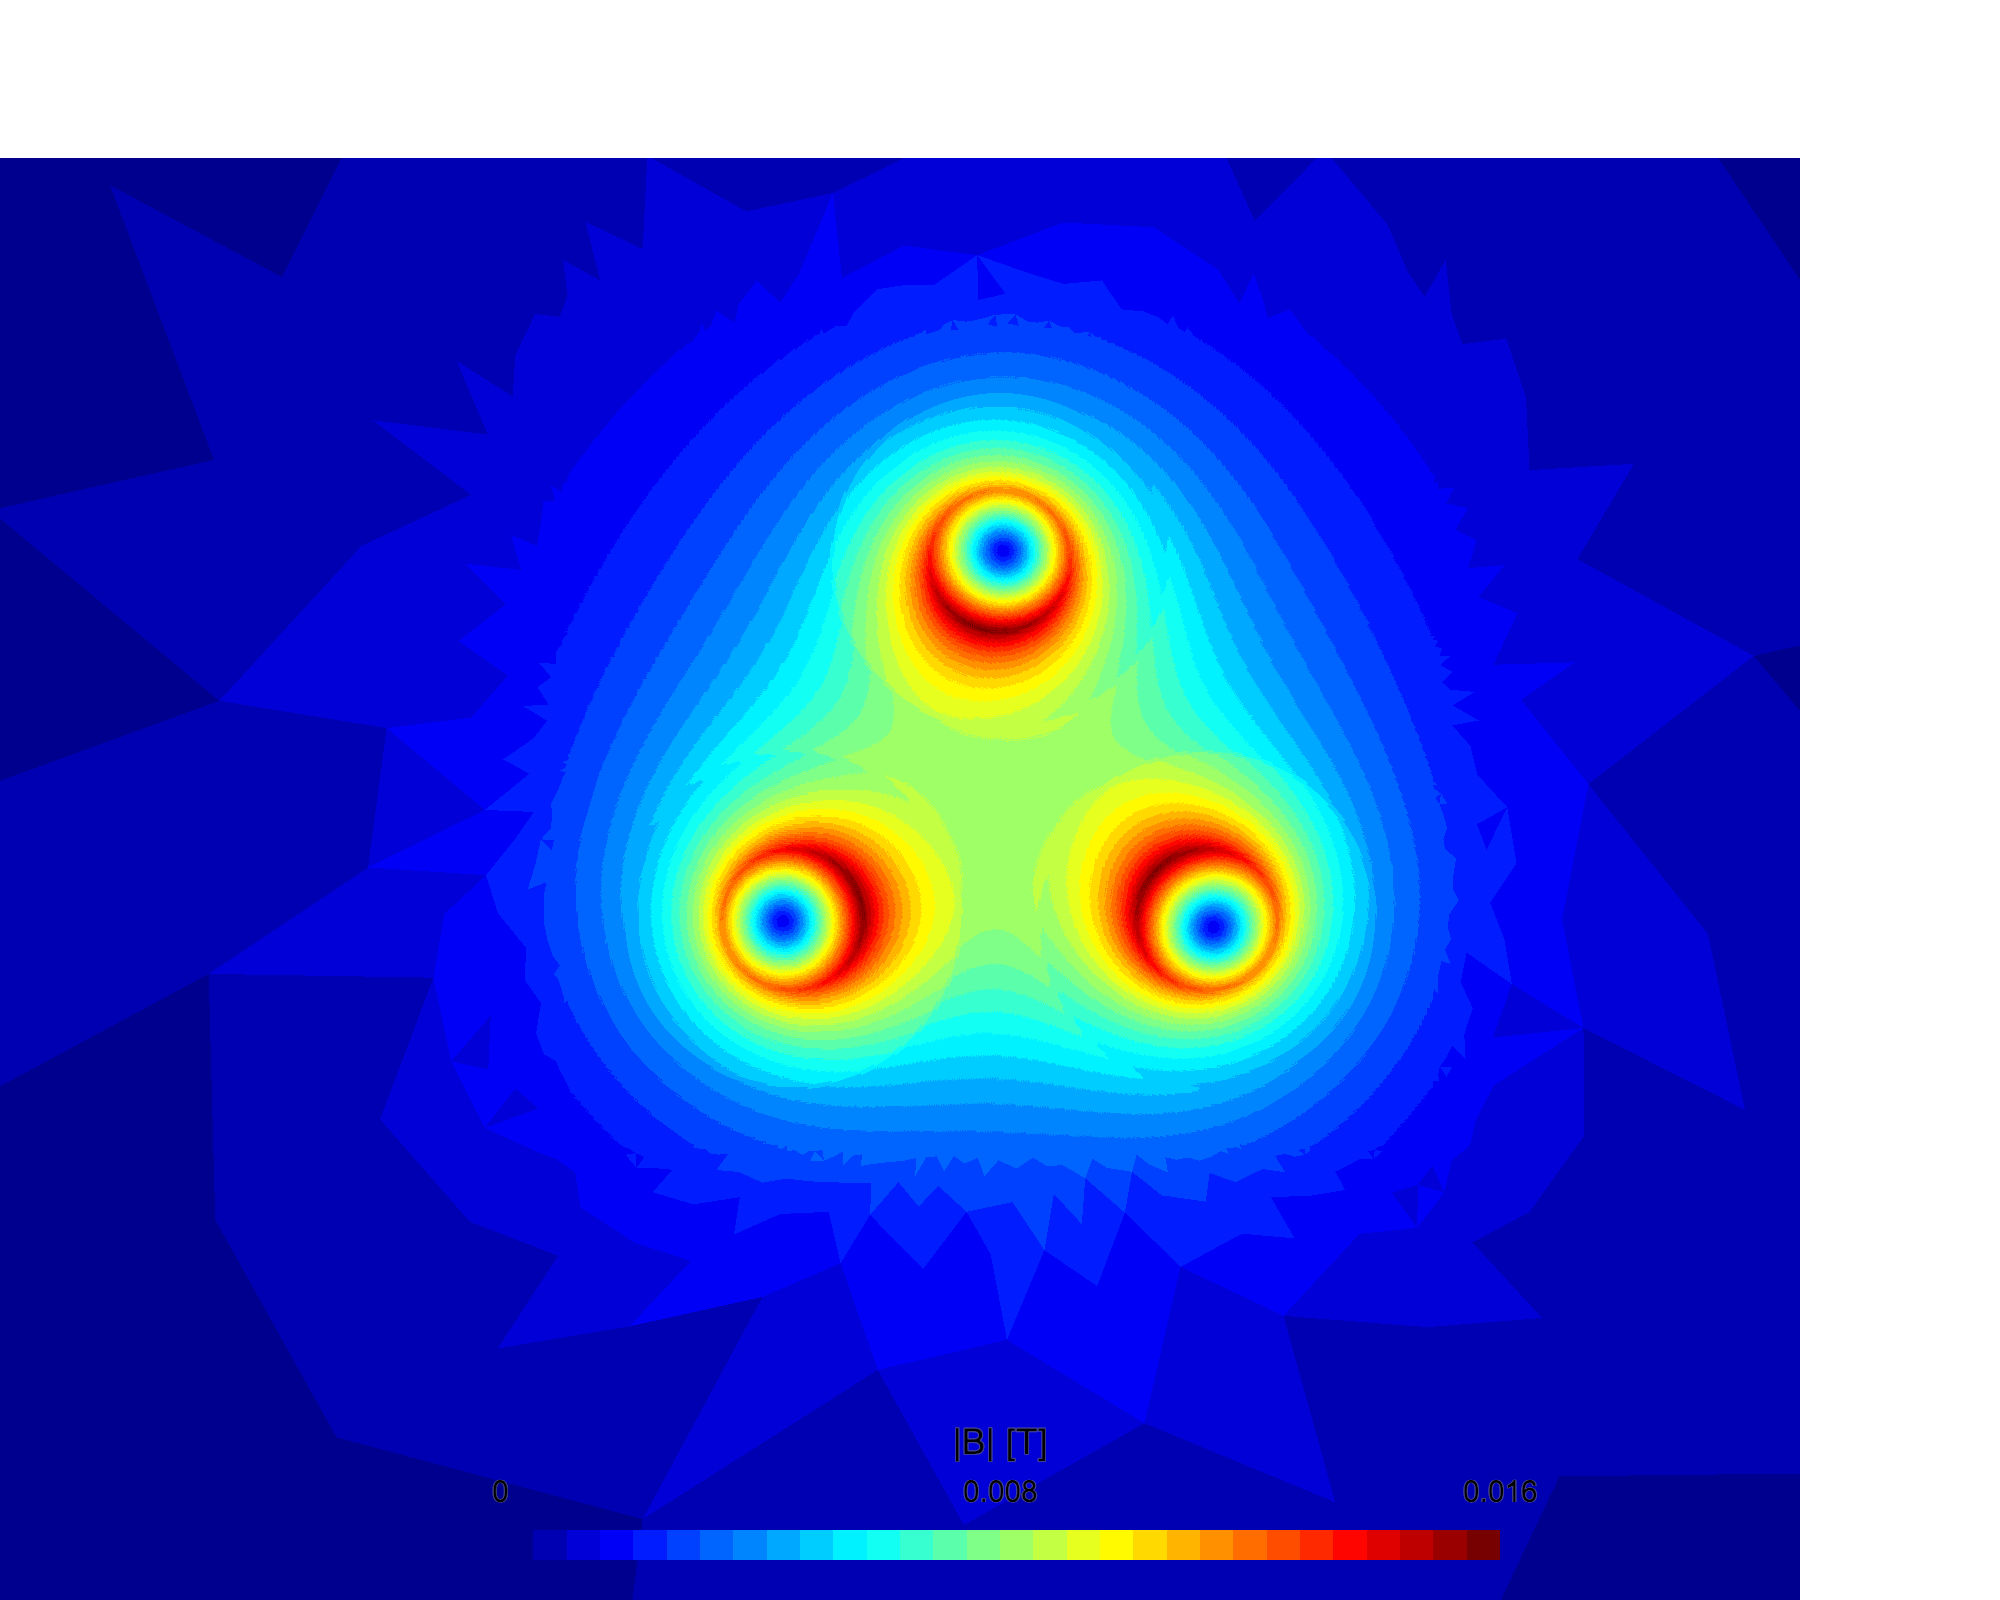
\includegraphics[width=0.62\linewidth]{m_b.png}\end{center}
Peak \(|\hat{\mathbf B}|\) is 15.6 mT, on the conductor surfaces facing the trefoil
centre (location (16.3, \(-7.5\)) mm on phase C; single-conductor estimate \(\mu_0\hat I/(2\pi r_c)=13.4\) mT, raised by the
neighbours). \(|\mathbf B|\) rises linearly inside each conductor, falls like \(1/r\)
in the insulation, and the balanced trefoil field decays quickly in the soil: at the box
edge it is below 1\% of its peak.

\codeguide{\mfile: \texttt{bm}, \texttt{Mag\_Maps}.}{Press \textbf{Run}.}
{\texttt{res/b\_norm.pos} (T, peak phasor norm).}

\section*{Q3.7 Current density}
\assignmentquestion{\QuestionThreeSeven}
\begin{center}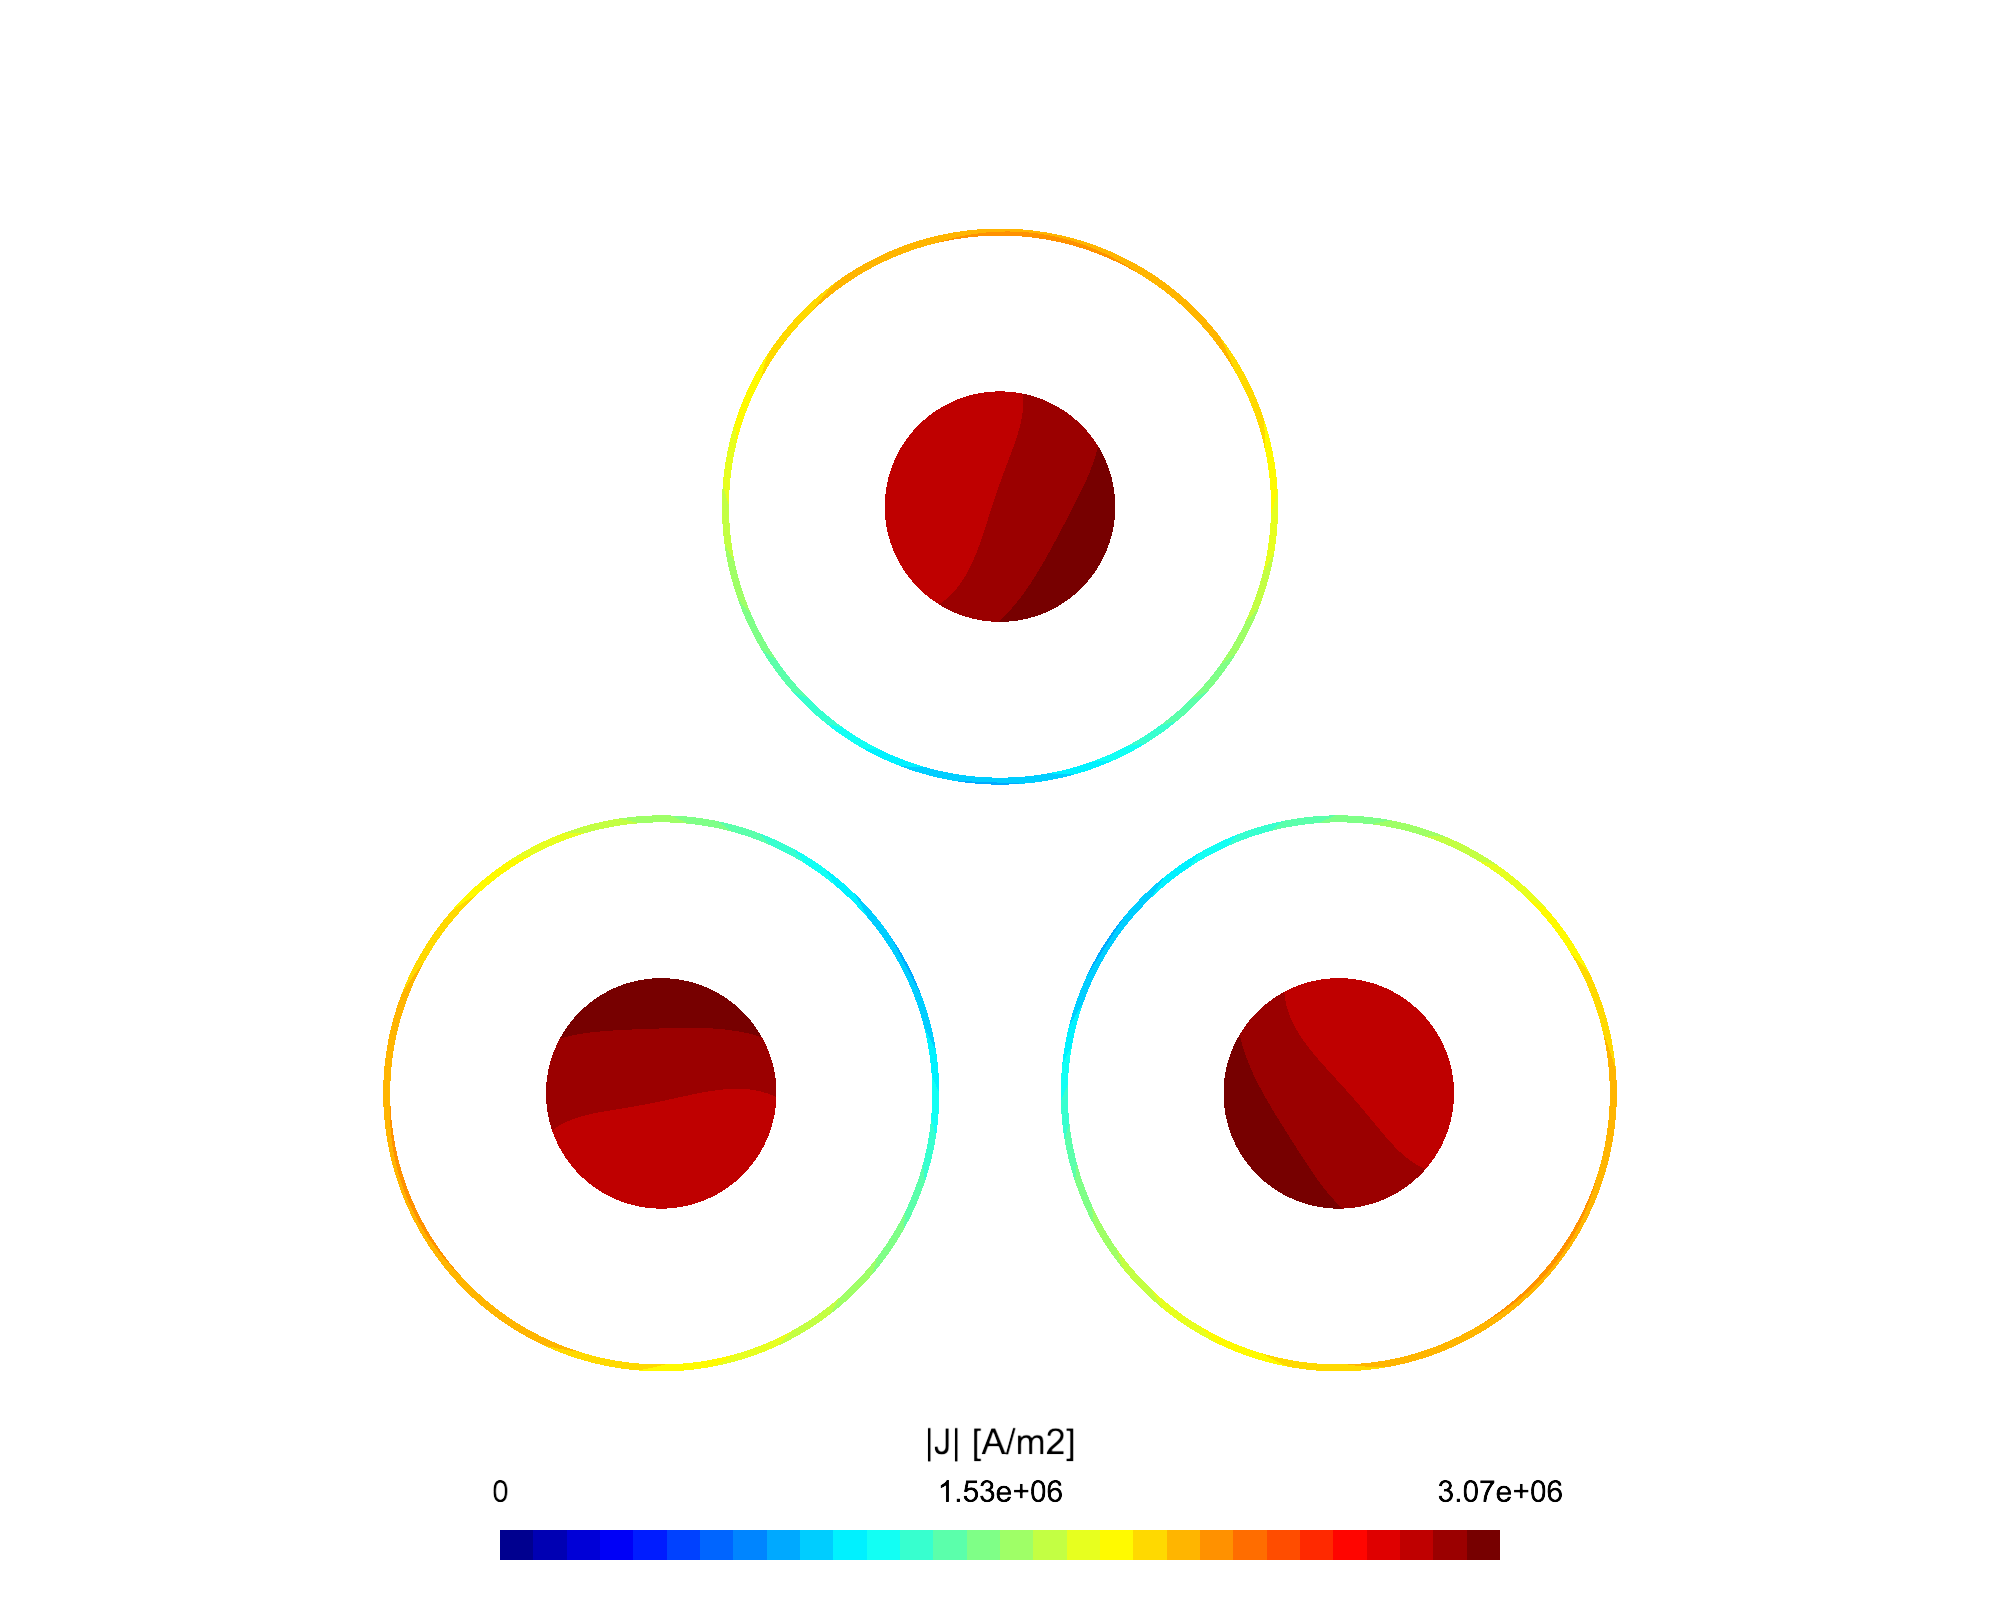
\includegraphics[width=0.48\linewidth]{m_j.png}\hfill
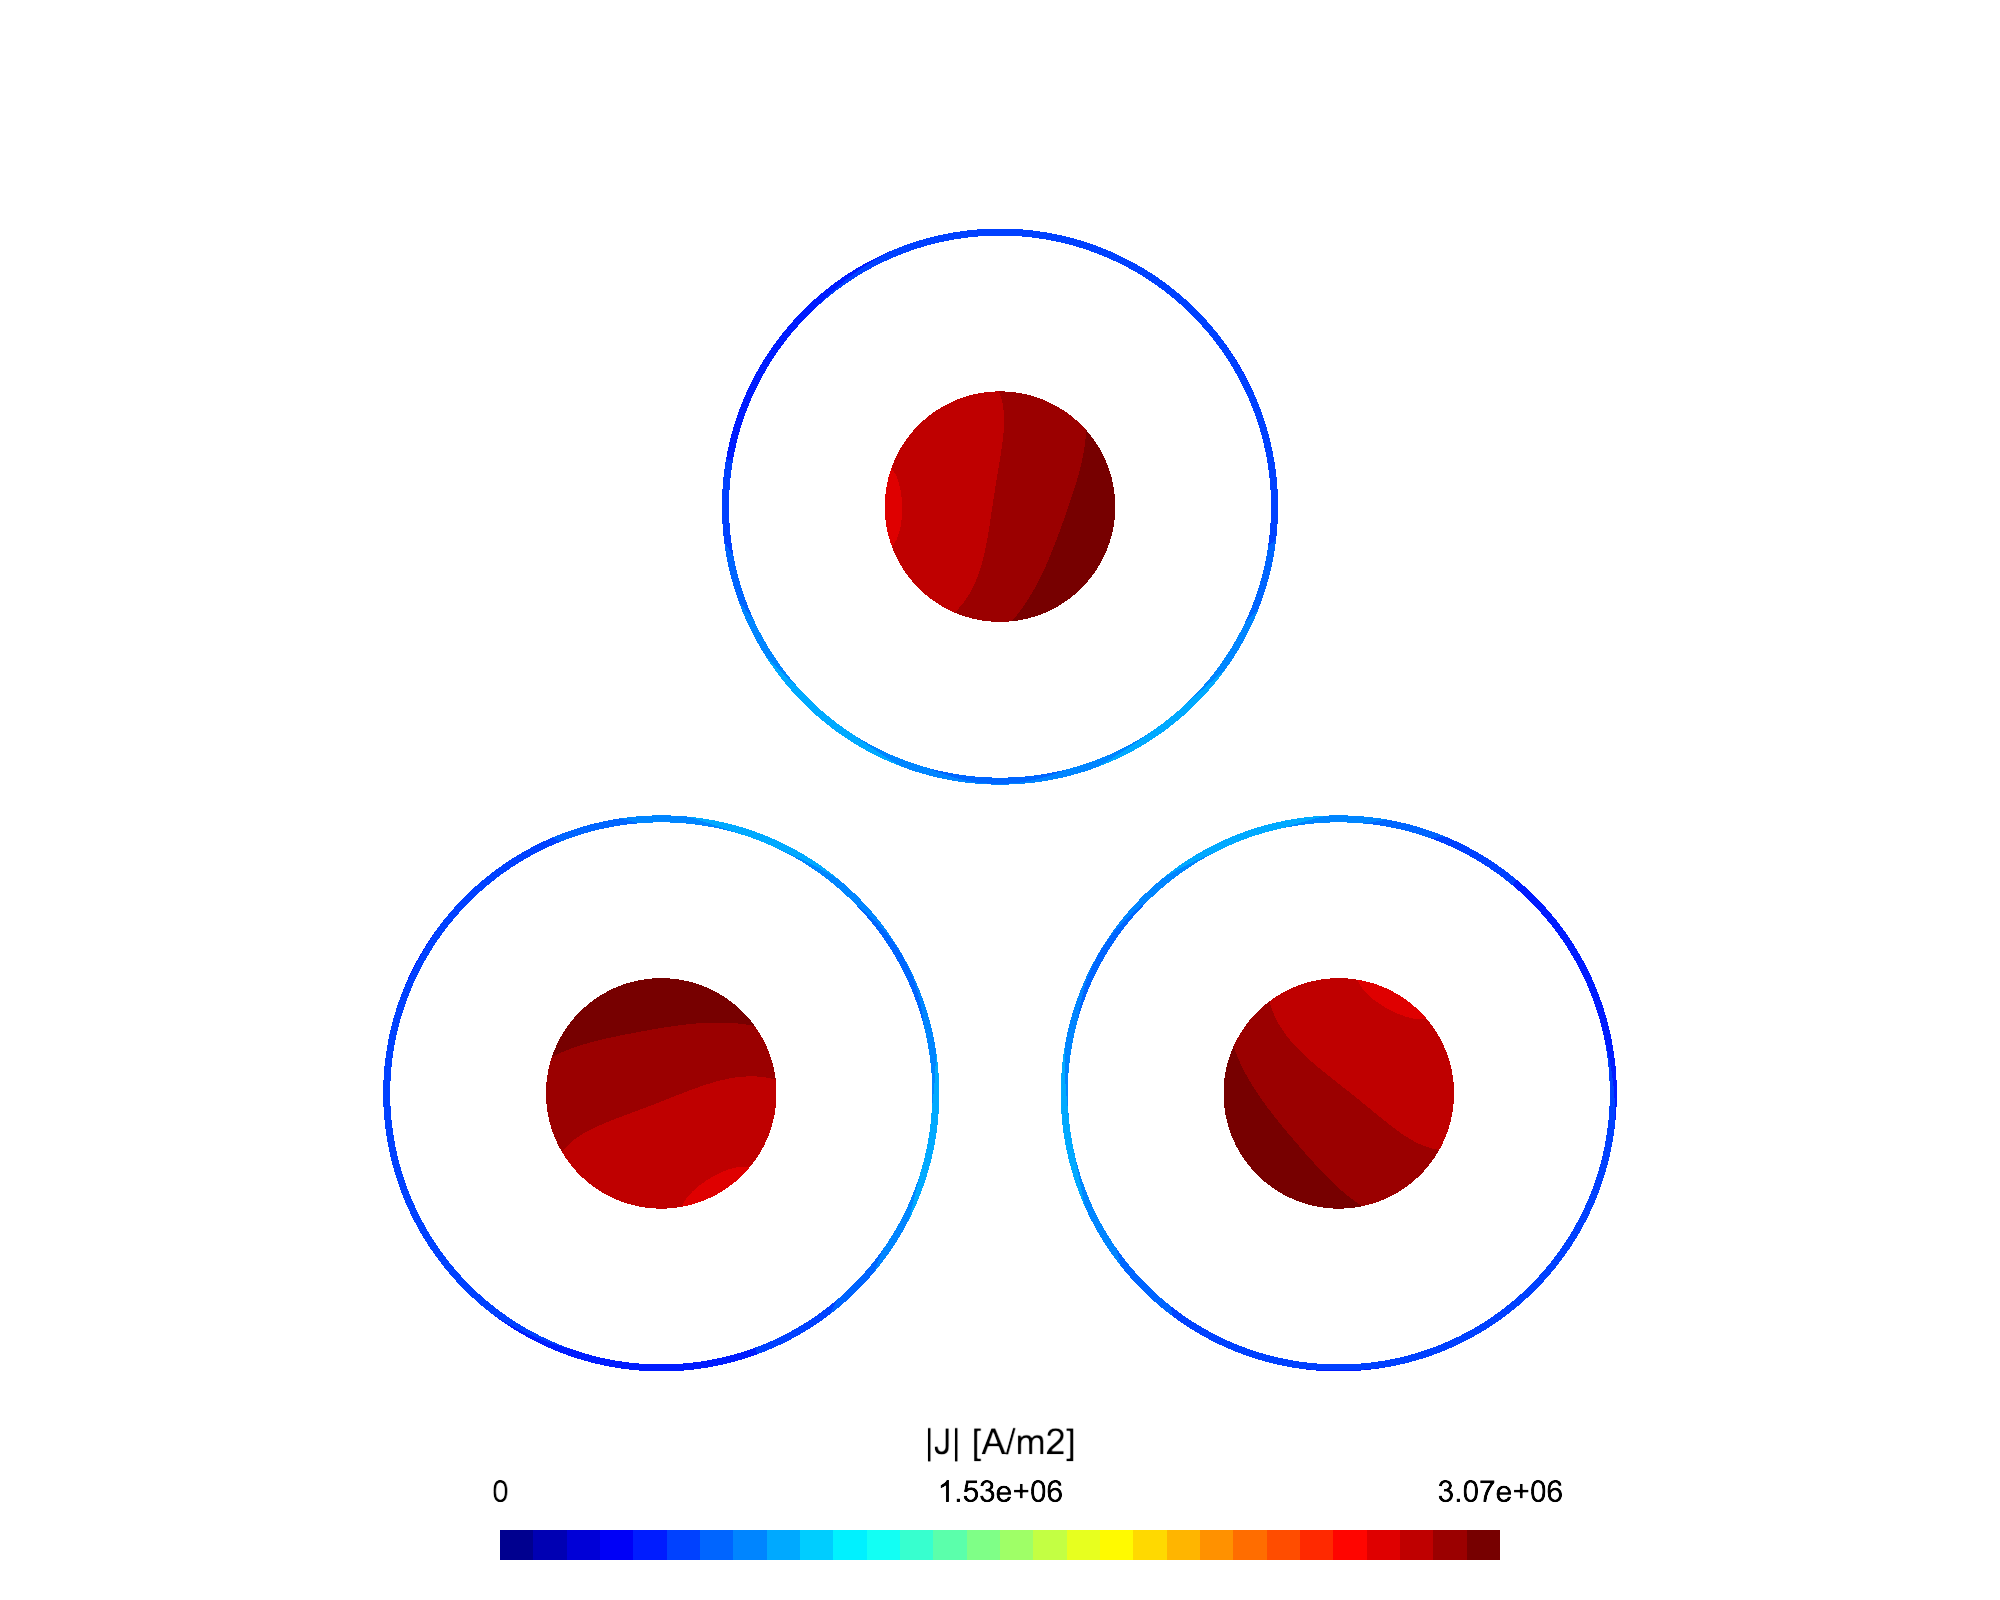
\includegraphics[width=0.48\linewidth]{m_j_single.png}\end{center}
Left: both-end bonding; right: single-point. Average conductor density
\(\hat I/A=2.88~\mathrm{A/mm^2}\) peak, maximum 3.07 A/mm\textsuperscript{2} at the
surface, on the side facing the next phase (proximity with 120\(^\circ\)-shifted currents). Screens: both-end bonded, the circulating current
(\(\approx\)1.6 A/mm\textsuperscript{2} peak) dominates; single-point, only local eddies remain
(opposite signs on the near and far sides of each ring, zero net current).

\codeguide{\mfile: \texttt{jm} (total current, including \(\mathbf u_r\)).}{Press \textbf{Run}.}
{\texttt{res/j\_norm.pos} (A/m\textsuperscript{2}, peak).}

\newpage
\section*{Q3.8 Joule losses per part}
\assignmentquestion{\QuestionThreeEight}
\(p=|\hat{\mathbf j}|^2/(2\sigma)\), integrated per region (W/m = kW/km), using the
\emph{total} current density \(-\sigma(j\omega\mathbf a+\mathbf u_r)\).
\begin{center}\small
\begin{tabular}{@{}lrrr@{}}\toprule
{[kW/km]} & Both ends & Single point & IEC 60287\\\midrule
Aluminium conductors (3) & \Pcbase & \Pcsingle & 60.55\\
Copper screens (3) & \Psbase & \Pssingle & 3.44\\
Armour / pipe & -- & -- & --\\
Environment (soil, \(\sigma=0\)) & 0 & 0 & --\\\midrule
Total & \Ptbase & \Ptsingle & 63.99\\\bottomrule
\end{tabular}
\end{center}
Each phase conductor loses 20.18 kW/km (symmetry of the trefoil to 0.0004\%).

\codeguide{\mfile: \texttt{Losses} and \texttt{Mag\_Global}.}{Press \textbf{Run}.}
{\texttt{res/losses\_conductors.dat}, \texttt{losses\_screens.dat}, \texttt{losses\_condA/B/C.dat}.}

\section*{Q3.9 AC resistance and loss separation}
\assignmentquestion{\QuestionThreeNine}
\(R_{AC}=P_{\rm tot}/(3I^2)\) with \(I=350\) A RMS.
\begin{center}\small
\begin{tabular}{@{}lrr@{}}\toprule
{[\(\Omega\)/km at 20\(^\circ\)C]} & FE & Reference\\\midrule
\(R_{DC}\) (FE at 0.01 Hz) & \Racfdc & 0.164 (NKT max.)\\
Conductors only (DC + skin + proximity) & \Rcbase & 0.16475 (IEC)\\
\(R_{AC}\), both ends (incl.\ screens) & \Racbase & 0.17411 (IEC)\\
\(R_{AC}\), single point & \Racsingle & --\\
Terminal check \(\Re(-U_A/I_A)\) & \Zrbase & --\\\bottomrule
\end{tabular}
\end{center}
Separation (both ends): \(R_{AC}=R_{DC}(1+0.45\%_{\rm skin+prox}+6.25\%_{\rm screens})\).
The skin/proximity part is 0.45\%; the screen circulating and eddy losses add 6.25\%.
NKT gives no AC resistance; its \(R_{DC}=0.164~\Omega\)/km is met by construction of
\(\sigma_{\rm Al}\) (Section 1). At 90\(^\circ\)C the resistances would be
\(1+\alpha\,70\approx1.27\) times higher (Section 4).

\codeguide{\mfile: \texttt{R\_ohm\_km}, \texttt{Zterm\_ohm\_km}.}
{Press \textbf{Run}; for \(R_{DC}\): \texttt{-setnumber Freq 0.01}.}
{\texttt{res/R\_conductors\_ohm\_km.dat}, \texttt{R\_ac\_ohm\_km.dat}, \texttt{Z\_terminal\_ohm\_km.dat}.}

\newpage
\section*{Q3.10 Three-phase inductance}
\assignmentquestion{\QuestionThreeTen}
\textbf{Definition.} For a balanced symmetric system, the per-phase (positive-sequence)
inductance \(L\) is the one for which \(U_k=Z\,I_k\) in every phase. The stored energy is then
\(W=\tfrac34L\hat I^2=\tfrac14\int\nu|\hat{\mathbf b}|^2dA\), so
\(L=\int\nu|\hat{\mathbf b}|^2dA/(3\hat I^2)\). It includes internal inductance and the
reaction of the screen currents. Check: terminal \(\Im(-U_A/I_A)/\omega\) gives
0.3942 mH/km (0.05\% from the energy value).
\begin{center}\small
\begin{tabular}{@{}lrrrr@{}}\toprule
Frequency [Hz] & 0.01 & 5 & 50 & 500\\\midrule
\(L\) [mH/km] & \Lfdc & \Lffive & \Lbase & \Lfhund\\
\(R_{AC}\) [\(\Omega\)/km] & \Racfdc & \Racffive & \Racbase & \Racfhund\\\bottomrule
\end{tabular}
\end{center}
\textbf{Frequency dependence: yes.} With \(\mu\) constant, \(L\) still decreases with
frequency because the induced screen currents (\(\propto\omega\) at low frequency) and
eddy currents oppose the flux: \(-1.8\%\) from DC to 50 Hz, \(-35\%\) at 500 Hz.
With single-point bonding the 50 Hz value is \Lsingle\ mH/km.

\textbf{Comparison.} Datasheet: \(X=0.12~\Omega\)/km (trefoil, touching)
\(\Rightarrow L=0.382\) mH/km. FE touching: \Ltouching\ mH/km (+2.6\%, the datasheet
value is rounded to two digits: \(0.115\le X<0.125\) gives 0.366--0.398 mH/km, which
includes the FE). Analytical \(2\,10^{-7}\ln(s/(r_ce^{-1/4}))\) without screens:
0.4043 mH/km, vs FE single-point \Lsingle\ (\(-1.0\%\)).

\codeguide{\mfile: \texttt{L\_mH\_km}, \texttt{Zterm\_ohm\_km}.}{\texttt{-setnumber Freq 5/500/0.01}.}
{\texttt{res/L\_mH\_km.dat}.}

\section*{Q3.11 Loss reduction: single-point (or cross-) bonding}
\assignmentquestion{\QuestionThreeEleven}
\begin{center}\def\figw{0.55\linewidth}\def\figh{5cm}\def\datadir{data}
% Shared pgfplots style for the report and the slides. \figw / \figh set the size.
\providecommand{\figw}{0.95\linewidth}\providecommand{\figh}{5.2cm}
\providecommand{\datadir}{data}
\ifdefined\figwlen\else\newlength\figwlen\fi\setlength{\figwlen}{\figw}
\pgfplotsset{every axis/.append style={width=\figw,height=\figh,grid=major,
  grid style={gray!25},tick label style={font=\scriptsize},label style={font=\small},
  legend style={font=\scriptsize,draw=none,fill=white,fill opacity=0.85,text opacity=1}}}
\definecolor{cA}{HTML}{254C58}\definecolor{cB}{HTML}{D1495B}\definecolor{cC}{HTML}{EDAE49}
% Q3.11: losses per km for both-end vs single-point bonding (massive Al, 350 A, 20 C).
\begin{tikzpicture}\begin{axis}[xbar stacked,bar width=14pt,xmin=0,xmax=78,clip=false,
  xlabel={Losses [kW/km]},ytick={1,2},yticklabels={Single point,Both ends},ymin=0.4,ymax=2.6,
  legend style={at={(0.5,1.03)},anchor=south,legend columns=2}]
\addplot[fill=cA!80,draw=none] coordinates {(\Pcsingle,1) (\Pcbase,2)};
\addplot[fill=cB!90,draw=none] coordinates {(\Pssingle,1) (\Psbase,2)};
\legend{Al conductors,Cu screens}
\node[font=\scriptsize,anchor=west] at (axis cs:\Ptbase,2) {\Ptbase};
\node[font=\scriptsize,anchor=west] at (axis cs:\Ptsingle,1) {\Ptsingle};
\end{axis}\end{tikzpicture}
\end{center}
Opening the screen loop at one end removes the circulating current: total losses drop
from \Ptbase\ to \Ptsingle\ kW/km (\(-5.0\%\)), \(R_{AC}\) from \Racbase\ to \Racsingle\
\(\Omega\)/km. The same holds for cross-bonding over three equal minor sections.
Cost: a standing screen voltage at the open end, \(|U|\,\ell\) with
\(|U|=19.5~\mathrm{V/km}\) RMS per phase at 350 A (FE; the estimate \(X I=19.9\) V/km agrees),
which limits the single-point section length (touch-voltage limits, sheath voltage limiters at the open end).
Because the conductor loss dominates (94\%), the gain is modest for this cable; NKT
indeed gives the same 350 A for both bondings in touching trefoil. The thermal
benefit is quantified in Section 4.

\codeguide{\mfile: \texttt{Flag\_Bonding}.}{\texttt{-setnumber Flag\_Bonding 1}.}
{\texttt{res/losses\_screens.dat}, \texttt{res/voltages\_V\_m.dat}.}

\subsection*{Sources}
\small
\textbf{[IEC]} IEC 60287-1-1, \emph{Electric cables -- Calculation of the current rating},
\S2.1.2--2.1.4 (\(y_s\), \(y_p\)) and \S2.3.1 (\(\lambda_1'\), single-core cables in trefoil,
both ends bonded). Local \href{../NMES_Assignment_2026.pdf}{NMES Assignment 2026},
Appendices A--B; local \href{../Datasheet 33 kV single core cable XLPE-AL.pdf}{NKT datasheet}, pp.19--20
(solid conductor, \(R_{DC}\), 50 Hz reactance, ratings). Material data: Section 1, Q1.1.
Gmsh 4.15.2, GetDP 4.0.0-git-259f4c38.
\end{document}
